\documentclass[twoside]{book}

% Packages required by doxygen
\usepackage{fixltx2e}
\usepackage{calc}
\usepackage{doxygen}
\usepackage[export]{adjustbox} % also loads graphicx
\usepackage{graphicx}
\usepackage[utf8]{inputenc}
\usepackage{makeidx}
\usepackage{multicol}
\usepackage{multirow}
\PassOptionsToPackage{warn}{textcomp}
\usepackage{textcomp}
\usepackage[nointegrals]{wasysym}
\usepackage[table]{xcolor}

% Font selection
\usepackage[T1]{fontenc}
\usepackage[scaled=.90]{helvet}
\usepackage{courier}
\usepackage{amssymb}
\usepackage{sectsty}
\renewcommand{\familydefault}{\sfdefault}
\allsectionsfont{%
  \fontseries{bc}\selectfont%
  \color{darkgray}%
}
\renewcommand{\DoxyLabelFont}{%
  \fontseries{bc}\selectfont%
  \color{darkgray}%
}
\newcommand{\+}{\discretionary{\mbox{\scriptsize$\hookleftarrow$}}{}{}}

% Page & text layout
\usepackage{geometry}
\geometry{%
  a4paper,%
  top=2.5cm,%
  bottom=2.5cm,%
  left=2.5cm,%
  right=2.5cm%
}
\tolerance=750
\hfuzz=15pt
\hbadness=750
\setlength{\emergencystretch}{15pt}
\setlength{\parindent}{0cm}
\setlength{\parskip}{3ex plus 2ex minus 2ex}
\makeatletter
\renewcommand{\paragraph}{%
  \@startsection{paragraph}{4}{0ex}{-1.0ex}{1.0ex}{%
    \normalfont\normalsize\bfseries\SS@parafont%
  }%
}
\renewcommand{\subparagraph}{%
  \@startsection{subparagraph}{5}{0ex}{-1.0ex}{1.0ex}{%
    \normalfont\normalsize\bfseries\SS@subparafont%
  }%
}
\makeatother

% Headers & footers
\usepackage{fancyhdr}
\pagestyle{fancyplain}
\fancyhead[LE]{\fancyplain{}{\bfseries\thepage}}
\fancyhead[CE]{\fancyplain{}{}}
\fancyhead[RE]{\fancyplain{}{\bfseries\leftmark}}
\fancyhead[LO]{\fancyplain{}{\bfseries\rightmark}}
\fancyhead[CO]{\fancyplain{}{}}
\fancyhead[RO]{\fancyplain{}{\bfseries\thepage}}
\fancyfoot[LE]{\fancyplain{}{}}
\fancyfoot[CE]{\fancyplain{}{}}
\fancyfoot[RE]{\fancyplain{}{\bfseries\scriptsize Generated by Doxygen }}
\fancyfoot[LO]{\fancyplain{}{\bfseries\scriptsize Generated by Doxygen }}
\fancyfoot[CO]{\fancyplain{}{}}
\fancyfoot[RO]{\fancyplain{}{}}
\renewcommand{\footrulewidth}{0.4pt}
\renewcommand{\chaptermark}[1]{%
  \markboth{#1}{}%
}
\renewcommand{\sectionmark}[1]{%
  \markright{\thesection\ #1}%
}

% Indices & bibliography
\usepackage{natbib}
\usepackage[titles]{tocloft}
\setcounter{tocdepth}{3}
\setcounter{secnumdepth}{5}
\makeindex

% Custom commands
\newcommand{\clearemptydoublepage}{%
  \newpage{\pagestyle{empty}\cleardoublepage}%
}

\usepackage{caption}
\captionsetup{labelsep=space,justification=centering,font={bf},singlelinecheck=off,skip=4pt,position=top}

%===== C O N T E N T S =====

\begin{document}

% Titlepage & ToC
\pagenumbering{alph}
\begin{titlepage}
\vspace*{7cm}
\begin{center}%
{\Large Error\+Codes }\\
\vspace*{1cm}
{\large Generated by Doxygen 1.8.13}\\
\end{center}
\end{titlepage}
\clearemptydoublepage
\pagenumbering{roman}
\tableofcontents
\clearemptydoublepage
\pagenumbering{arabic}

%--- Begin generated contents ---
\chapter{Error Codes in C++ 11}
\label{md__r_e_a_d_m_e}
This project implements error codes in C++ 11 as an exercise.

\subsection*{Error Detection and Correction}

Error codes are algorithms that ensure the integrity of binary data. When data travels through arbitrary media through space (like in communication systems), or through time (like in storage/database systems), there is always the possibility that some of the information bits could get corrupted and flipped. With the use of error correction algorithms, it is possible to add some extra bits of information to the raw data so that if some corruptions were to occur, they can be detected. Using these extra error correction bits, it can also be possible to correct any errors that may have occured, and retrieve the uncorrupted raw data.

\subsubsection*{Implementation\+:}

In this implementation, the communication medium is a U\+DP channel. The product of this project is one executable -\/ error\+\_\+coder. This executable can be used either as a client or blocking server. The udp client takes string inputs from the command line, encodes them according to a user-\/specified error\+\_\+coding algorithm, and transmits them to the U\+DP server.

The U\+DP server, if alive, will recieve the coded message, detect the chosen error coding scheme, and then decode the original message. This decoded message is written to the console.

The following are the implemented error detection/correction codes


\begin{DoxyItemize}
\item {\tt Hamming (7, 3)}

Currently only detecting but not correcting errors.
\end{DoxyItemize}

\subsection*{Getting Started}

\subsubsection*{Core Services}

The core error coding services come from the executable \char`\"{}error\+\_\+coder\char`\"{}. There is a python script \char`\"{}kickoff\char`\"{} that delegates some C\+LI calls. You can start and stop the server with kickoff. But sending messages to the U\+DP server has to be done through the executble.

The {\bfseries kickoff} script acts as a clean command line interface to error\+\_\+coder. The following are the supported commands\+:


\begin{DoxyItemize}
\item --start [ --s, -\/s, -\/start]\+: A flag requesting to start the server.
\item --stop [ --e, -\/e, -\/end, --end]\+: A flag requesting to stop the server.
\item --p\+: The port to run the server and client on.
\item --l [-\/l, --logfile, -\/logile]\+: The path to the logfile where the output from the U\+DP server would go.
\item --c [--clear]\+: A flag requesting to clear the U\+DP server logfile.
\end{DoxyItemize}

The {\bfseries error\+\_\+coder} application also accepts command-\/line inputs. The following are the supported commands\+:


\begin{DoxyItemize}
\item --p\+: The port to run the server/client on.
\item --m\+: A number signifying which mode to run error\+\_\+coder in. 1 = Client, 2 = Server.
\item --i\+: A string/sequence of characters\+: The string message to encode and transmit if running error\+\_\+coder in client mode.
\item --c\+: The error code to use. 1 = clear text. 2 = Hamming(7,4)
\end{DoxyItemize}

\subsubsection*{Installing}

make pre -\/ Install all the needed dependancies

make clean all -\/ Build the project

sudo make install -\/ install error\+\_\+coder to /usr/local/bin

\subsection*{Examples}

\subsubsection*{Starting the U\+DP listener server on 8888 (background + logfile)}

./kickoff --start --p 8888

Note that even though error\+\_\+coder \textquotesingle{}s U\+DP server is blocking, calling it through kickoff runs it in the background and traps the logs to a configurable path (Defaults to /tmp/error\+\_\+correction\+\_\+server.log)

\subsubsection*{Starting the U\+DP listener server on 8888 (foreground + console logs)}

error\+\_\+coder --p 8888 --m 2

\subsubsection*{Ending the U\+DP listener server (non blocking)}

./kickoff --stop

\subsubsection*{Send an error encoded message to the U\+DP server -\/ Clear (blocking)}

This is an example of sending the phrase \char`\"{}\+Hola\char`\"{} to the U\+DP server where each byte is sent without encoding.

error\+\_\+coder --p 8888 --m 1 --c 1 --i Hola

\subsubsection*{Send an error encoded message to the U\+DP server -\/ Hamming (blocking)}

This is an example of sending the phrase \char`\"{}\+Hello\char`\"{} to the U\+DP server where each byte is encoded with Hamming (7, 4) coding

error\+\_\+coder --p 8888 --m 1 --c 2 --i Hello

\subsubsection*{Clear the log files (blocking)}

./kickoff --clear

\subsubsection*{Tail the log files}

tail -\/f /tmp/error\+\_\+correction\+\_\+server.log 
\chapter{Hierarchical Index}
\section{Class Hierarchy}
This inheritance list is sorted roughly, but not completely, alphabetically\+:\begin{DoxyCompactList}
\item \contentsline{section}{Bilbo}{\pageref{class_bilbo}}{}
\item \contentsline{section}{Encoded\+Message}{\pageref{struct_encoded_message}}{}
\item \contentsline{section}{i\+Logggable}{\pageref{classi_logggable}}{}
\begin{DoxyCompactList}
\item \contentsline{section}{Encoder}{\pageref{class_encoder}}{}
\item \contentsline{section}{Udp\+Client}{\pageref{class_udp_client}}{}
\item \contentsline{section}{Udp\+Server}{\pageref{class_udp_server}}{}
\end{DoxyCompactList}
\end{DoxyCompactList}

\chapter{Class Index}
\section{Class List}
Here are the classes, structs, unions and interfaces with brief descriptions\+:\begin{DoxyCompactList}
\item\contentsline{section}{\textbf{ Bilbo} \\*General utilties }{\pageref{class_bilbo}}{}
\item\contentsline{section}{\textbf{ Encoded\+Message} \\*The struct that contains data that encapsulates the encoding type and the encoded message }{\pageref{struct_encoded_message}}{}
\item\contentsline{section}{\textbf{ Encoder} \\*The class that conducts error coding of string messages }{\pageref{class_encoder}}{}
\item\contentsline{section}{\textbf{ i\+Logggable} }{\pageref{classi_logggable}}{}
\item\contentsline{section}{\textbf{ Udp\+Client} }{\pageref{class_udp_client}}{}
\item\contentsline{section}{\textbf{ Udp\+Server} }{\pageref{class_udp_server}}{}
\end{DoxyCompactList}

\chapter{Class Documentation}
\section{Bilbo Class Reference}
\label{class_bilbo}\index{Bilbo@{Bilbo}}


General utilties.  




{\ttfamily \#include $<$utils.\+h$>$}

\subsection*{Public Member Functions}
\begin{DoxyCompactItemize}
\item 
bool \textbf{ read\+Text\+File} (const char $\ast$path, std\+::string \&input\+Data)
\item 
int \textbf{ fast\+\_\+atoi} (const char $\ast$str)
\begin{DoxyCompactList}\small\item\em String to integer conversion. \end{DoxyCompactList}\item 
std\+::unordered\+\_\+map$<$ std\+::string, std\+::string $>$ \textbf{ get\+Key\+Value\+Pairs} (const std\+::string \&input, const char split\+Token, const char equality)
\begin{DoxyCompactList}\small\item\em Get the Key Value Pairs. \end{DoxyCompactList}\item 
std\+::vector$<$ std\+::string $>$ \textbf{ split} (const std\+::string \&input, const char delimiter)
\begin{DoxyCompactList}\small\item\em Split a string by a delimiter. \end{DoxyCompactList}\item 
void \textbf{ cli} (const int argc, const char $\ast$$\ast$arguments, std\+::unordered\+\_\+map$<$ std\+::string, std\+::string $>$ \&kv)
\begin{DoxyCompactList}\small\item\em Extract key value pairs from the command line and pass it into a string map. \end{DoxyCompactList}\end{DoxyCompactItemize}


\subsection{Detailed Description}
General utilties. 

\subsection{Member Function Documentation}
\mbox{\label{class_bilbo_ae13bf7c5b889b3fdf8077fa9733ea1d7}} 
\index{Bilbo@{Bilbo}!cli@{cli}}
\index{cli@{cli}!Bilbo@{Bilbo}}
\subsubsection{cli()}
{\footnotesize\ttfamily void Bilbo\+::cli (\begin{DoxyParamCaption}\item[{const int}]{argc,  }\item[{const char $\ast$$\ast$}]{arguments,  }\item[{std\+::unordered\+\_\+map$<$ std\+::string, std\+::string $>$ \&}]{kv }\end{DoxyParamCaption})}



Extract key value pairs from the command line and pass it into a string map. 


\begin{DoxyParams}{Parameters}
{\em argc} & \\
\hline
{\em arguments} & \\
\hline
{\em kv} & \\
\hline
\end{DoxyParams}
\mbox{\label{class_bilbo_a4c567f47e8f57e753b18b5ed8fcdba8b}} 
\index{Bilbo@{Bilbo}!fast\+\_\+atoi@{fast\+\_\+atoi}}
\index{fast\+\_\+atoi@{fast\+\_\+atoi}!Bilbo@{Bilbo}}
\subsubsection{fast\+\_\+atoi()}
{\footnotesize\ttfamily int Bilbo\+::fast\+\_\+atoi (\begin{DoxyParamCaption}\item[{const char $\ast$}]{str }\end{DoxyParamCaption})}



String to integer conversion. 


\begin{DoxyParams}{Parameters}
{\em str} & A const reference to the begeining of the string \\
\hline
\end{DoxyParams}
\begin{DoxyReturn}{Returns}
int The string converted to integer 
\end{DoxyReturn}
\mbox{\label{class_bilbo_a794461f514f95d4e45e3cab13013c82c}} 
\index{Bilbo@{Bilbo}!get\+Key\+Value\+Pairs@{get\+Key\+Value\+Pairs}}
\index{get\+Key\+Value\+Pairs@{get\+Key\+Value\+Pairs}!Bilbo@{Bilbo}}
\subsubsection{get\+Key\+Value\+Pairs()}
{\footnotesize\ttfamily std\+::unordered\+\_\+map$<$ std\+::string, std\+::string $>$ Bilbo\+::get\+Key\+Value\+Pairs (\begin{DoxyParamCaption}\item[{const std\+::string \&}]{input,  }\item[{const char}]{split\+Token,  }\item[{const char}]{equality }\end{DoxyParamCaption})}



Get the Key Value Pairs. 


\begin{DoxyParams}{Parameters}
{\em input} & A const string to split \\
\hline
{\em split\+Token} & The line separator \\
\hline
{\em equality} & The separator between keys and values \\
\hline
\end{DoxyParams}
\begin{DoxyReturn}{Returns}
std\+::unordered\+\_\+map$<$ std\+::string, std\+::string$>$ 
\end{DoxyReturn}
\mbox{\label{class_bilbo_a62d8043f94ac512b6f2851c96e4fa441}} 
\index{Bilbo@{Bilbo}!read\+Text\+File@{read\+Text\+File}}
\index{read\+Text\+File@{read\+Text\+File}!Bilbo@{Bilbo}}
\subsubsection{read\+Text\+File()}
{\footnotesize\ttfamily bool Bilbo\+::read\+Text\+File (\begin{DoxyParamCaption}\item[{const char $\ast$}]{path,  }\item[{std\+::string \&}]{input\+Data }\end{DoxyParamCaption})}

Reads the data from the text file specified in the path and puts it inside the string 
\begin{DoxyParams}{Parameters}
{\em path} & Path to the text file \\
\hline
{\em input\+Data} & The std\+:string into which the file content will be written \\
\hline
\end{DoxyParams}
\begin{DoxyReturn}{Returns}
The truth whether the read worked correctly. 
\end{DoxyReturn}
\mbox{\label{class_bilbo_abbafbc1117d01287115c7ebd08114c59}} 
\index{Bilbo@{Bilbo}!split@{split}}
\index{split@{split}!Bilbo@{Bilbo}}
\subsubsection{split()}
{\footnotesize\ttfamily std\+::vector$<$ std\+::string $>$ Bilbo\+::split (\begin{DoxyParamCaption}\item[{const std\+::string \&}]{input,  }\item[{const char}]{delimiter }\end{DoxyParamCaption})}



Split a string by a delimiter. 


\begin{DoxyParams}{Parameters}
{\em input} & A const string to split \\
\hline
{\em delimiter} & The const character to split the string by \\
\hline
\end{DoxyParams}
\begin{DoxyReturn}{Returns}
std\+::vector$<$std\+::string$>$ 
\end{DoxyReturn}


The documentation for this class was generated from the following files\+:\begin{DoxyCompactItemize}
\item 
headers/utils.\+h\item 
utils.\+cpp\end{DoxyCompactItemize}

\section{Encoded\+Message Struct Reference}
\label{struct_encoded_message}\index{Encoded\+Message@{Encoded\+Message}}


The struct that contains data that encapsulates the encoding type and the encoded message.  




{\ttfamily \#include $<$encoder.\+h$>$}

\subsection*{Public Member Functions}
\begin{DoxyCompactItemize}
\item 
\mbox{\label{struct_encoded_message_a5993f82f3db6caff8924f5031b266f09}} 
{\bfseries Encoded\+Message} (const char $\ast$m)
\end{DoxyCompactItemize}
\subsection*{Public Attributes}
\begin{DoxyCompactItemize}
\item 
\mbox{\label{struct_encoded_message_ab1b733ac5585e8ce61b81812e11c240f}} 
Encoding\+Type {\bfseries code}
\item 
\mbox{\label{struct_encoded_message_acfd5bc4448b8a2e3761d8c4a3995489a}} 
std\+::string {\bfseries message}
\end{DoxyCompactItemize}


\subsection{Detailed Description}
The struct that contains data that encapsulates the encoding type and the encoded message. 

The documentation for this struct was generated from the following file\+:\begin{DoxyCompactItemize}
\item 
headers/encoder.\+h\end{DoxyCompactItemize}

\section{Encoder Class Reference}
\label{class_encoder}\index{Encoder@{Encoder}}


The class that conducts error coding of string messages.  




{\ttfamily \#include $<$encoder.\+h$>$}



Inheritance diagram for Encoder\+:
\nopagebreak
\begin{figure}[H]
\begin{center}
\leavevmode
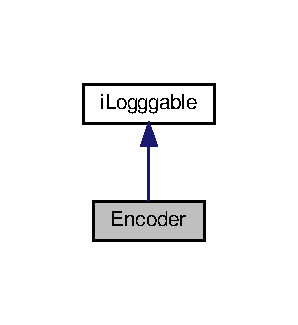
\includegraphics[width=143pt]{class_encoder__inherit__graph}
\end{center}
\end{figure}


Collaboration diagram for Encoder\+:
\nopagebreak
\begin{figure}[H]
\begin{center}
\leavevmode
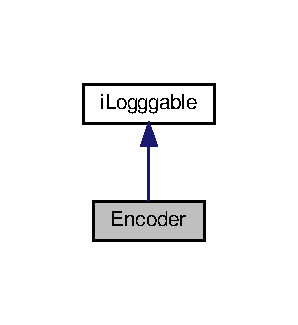
\includegraphics[width=143pt]{class_encoder__coll__graph}
\end{center}
\end{figure}
\subsection*{Public Member Functions}
\begin{DoxyCompactItemize}
\item 
\mbox{\label{class_encoder_abd165b5418381b066a4bfe70d41340a5}} 
{\bfseries Encoder} (const char $\ast$name)
\item 
unsigned char \textbf{ fourbit\+Hamming} (const unsigned char \&nibble)
\item 
unsigned char \textbf{ checkfourbit\+Hamming} (const unsigned char \&encoded\+\_\+byte)
\begin{DoxyCompactList}\small\item\em Checks the number of errors in a hamming coded byte. Hamming coded bytes contain 7 bits of information + 1 bit of padding. \end{DoxyCompactList}\item 
unsigned char \textbf{ reversfour\+Bit\+Hamming} (const unsigned char \&lower, const unsigned char \&upper)
\begin{DoxyCompactList}\small\item\em Combine two bytes of hamming (7,4) coded data to create the original message byte. \end{DoxyCompactList}\item 
void \textbf{ corrupt\+Nibble} (unsigned char \&buffer)
\begin{DoxyCompactList}\small\item\em Flip the bits in the lower nibble of the input byte reference. \end{DoxyCompactList}\item 
int \textbf{ get\+Encoding\+Count} ()
\begin{DoxyCompactList}\small\item\em Get the distinct number Encodings supported. \end{DoxyCompactList}\item 
void \textbf{ debug\+Byte} (const unsigned char \&d, const char $\ast$label)
\begin{DoxyCompactList}\small\item\em Print out the bits in a char. \end{DoxyCompactList}\item 
void \textbf{ decode\+\_\+hamming347} (const std\+::string \&input, std\+::string \&output)
\begin{DoxyCompactList}\small\item\em Decode Hamming 347 codes, Reads a C++ 11 string and assumes that each character has 7 bits of hamming (7, 4) and 1 padding bit. The 7 bits are assume to be an encoded form of an original message which contained 4 bits. \end{DoxyCompactList}\item 
\textbf{ Encoded\+Message} \textbf{ encode\+\_\+hamming347} (const std\+::string \&input)
\begin{DoxyCompactList}\small\item\em Encode Hamming 347 codes, Reads a C++ 11 string, splits each character into two pairs of 4 bits each, and performs Hamming (7, 4) error coding. \end{DoxyCompactList}\item 
\textbf{ Encoded\+Message} \textbf{ encode} (const std\+::string \&input, const Encoding\+Type \&enc\+Type)
\begin{DoxyCompactList}\small\item\em Encode a given message with the chosen error coding scheme. \end{DoxyCompactList}\item 
std\+::string \textbf{ encode\+To\+String} (const std\+::string \&input, const Encoding\+Type \&enc\+Type)
\begin{DoxyCompactList}\small\item\em Call the base encoder, composed. \end{DoxyCompactList}\item 
void \textbf{ decode} (const \textbf{ Encoded\+Message} \&rec)
\begin{DoxyCompactList}\small\item\em Detect the form of error coding the in the recieved messsage and perform error checking and correction. \end{DoxyCompactList}\item 
std\+::string \textbf{ compose} (const \textbf{ Encoded\+Message} \&message)
\begin{DoxyCompactList}\small\item\em convert a message struct into a message string. \end{DoxyCompactList}\item 
\textbf{ Encoded\+Message} \textbf{ decompose\+From\+Buffer} (const char $\ast$buffer, const int \&buffer\+Size)
\begin{DoxyCompactList}\small\item\em Extract the data struct from a char buffer of a known size. \end{DoxyCompactList}\end{DoxyCompactItemize}


\subsection{Detailed Description}
The class that conducts error coding of string messages. 

\subsection{Member Function Documentation}
\mbox{\label{class_encoder_a6986342c9a32104bcfd1257b4866ea3d}} 
\index{Encoder@{Encoder}!checkfourbit\+Hamming@{checkfourbit\+Hamming}}
\index{checkfourbit\+Hamming@{checkfourbit\+Hamming}!Encoder@{Encoder}}
\subsubsection{checkfourbit\+Hamming()}
{\footnotesize\ttfamily unsigned char Encoder\+::checkfourbit\+Hamming (\begin{DoxyParamCaption}\item[{const unsigned char \&}]{encoded\+\_\+byte }\end{DoxyParamCaption})}



Checks the number of errors in a hamming coded byte. Hamming coded bytes contain 7 bits of information + 1 bit of padding. 


\begin{DoxyParams}{Parameters}
{\em encoded\+\_\+byte} & The hamming coded byte of the form 0 p1 p2 p3 d1 d2 d3 d4, where pi are the parity bits, and di are the data bits \\
\hline
\end{DoxyParams}
\begin{DoxyReturn}{Returns}
unsigned char The number of errors detected. 
\end{DoxyReturn}
\mbox{\label{class_encoder_ac2f2f36d39af92e16c2442d9f013ce57}} 
\index{Encoder@{Encoder}!compose@{compose}}
\index{compose@{compose}!Encoder@{Encoder}}
\subsubsection{compose()}
{\footnotesize\ttfamily std\+::string Encoder\+::compose (\begin{DoxyParamCaption}\item[{const \textbf{ Encoded\+Message} \&}]{message }\end{DoxyParamCaption})}



convert a message struct into a message string. 


\begin{DoxyParams}{Parameters}
{\em message} & Encoding\+Message \\
\hline
\end{DoxyParams}
\begin{DoxyReturn}{Returns}
std\+::string One byte of encoding type + The message string 
\end{DoxyReturn}
\mbox{\label{class_encoder_a64893c2f29b0168c922fb003b2d67606}} 
\index{Encoder@{Encoder}!corrupt\+Nibble@{corrupt\+Nibble}}
\index{corrupt\+Nibble@{corrupt\+Nibble}!Encoder@{Encoder}}
\subsubsection{corrupt\+Nibble()}
{\footnotesize\ttfamily void Encoder\+::corrupt\+Nibble (\begin{DoxyParamCaption}\item[{unsigned char \&}]{buffer }\end{DoxyParamCaption})}



Flip the bits in the lower nibble of the input byte reference. 


\begin{DoxyParams}{Parameters}
{\em buffer} & The byte to corrupt the bits of. \\
\hline
\end{DoxyParams}
\mbox{\label{class_encoder_ad2535f1838162ef27e78942f13b8daf5}} 
\index{Encoder@{Encoder}!debug\+Byte@{debug\+Byte}}
\index{debug\+Byte@{debug\+Byte}!Encoder@{Encoder}}
\subsubsection{debug\+Byte()}
{\footnotesize\ttfamily void Encoder\+::debug\+Byte (\begin{DoxyParamCaption}\item[{const unsigned char \&}]{d,  }\item[{const char $\ast$}]{label }\end{DoxyParamCaption})}



Print out the bits in a char. 


\begin{DoxyParams}{Parameters}
{\em d} & The character byte to analyze \\
\hline
{\em label} & The label to print with the input \\
\hline
\end{DoxyParams}
\mbox{\label{class_encoder_a3c501051ae37446a8da8607010b02857}} 
\index{Encoder@{Encoder}!decode@{decode}}
\index{decode@{decode}!Encoder@{Encoder}}
\subsubsection{decode()}
{\footnotesize\ttfamily void Encoder\+::decode (\begin{DoxyParamCaption}\item[{const \textbf{ Encoded\+Message} \&}]{rec }\end{DoxyParamCaption})}



Detect the form of error coding the in the recieved messsage and perform error checking and correction. 


\begin{DoxyParams}{Parameters}
{\em rec} & message reciegved over the socket. \\
\hline
\end{DoxyParams}
\mbox{\label{class_encoder_a43d67d5174ff6a829a3fa093e447e538}} 
\index{Encoder@{Encoder}!decode\+\_\+hamming347@{decode\+\_\+hamming347}}
\index{decode\+\_\+hamming347@{decode\+\_\+hamming347}!Encoder@{Encoder}}
\subsubsection{decode\+\_\+hamming347()}
{\footnotesize\ttfamily void Encoder\+::decode\+\_\+hamming347 (\begin{DoxyParamCaption}\item[{const std\+::string \&}]{input,  }\item[{std\+::string \&}]{output }\end{DoxyParamCaption})}



Decode Hamming 347 codes, Reads a C++ 11 string and assumes that each character has 7 bits of hamming (7, 4) and 1 padding bit. The 7 bits are assume to be an encoded form of an original message which contained 4 bits. 


\begin{DoxyParams}{Parameters}
{\em input} & A constant string that doesn\textquotesingle{}t change \\
\hline
{\em output} & Where to write the decoded output to \\
\hline
\end{DoxyParams}
\mbox{\label{class_encoder_a6528526b6c98d8b8da669271a6daacd2}} 
\index{Encoder@{Encoder}!decompose\+From\+Buffer@{decompose\+From\+Buffer}}
\index{decompose\+From\+Buffer@{decompose\+From\+Buffer}!Encoder@{Encoder}}
\subsubsection{decompose\+From\+Buffer()}
{\footnotesize\ttfamily \textbf{ Encoded\+Message} Encoder\+::decompose\+From\+Buffer (\begin{DoxyParamCaption}\item[{const char $\ast$}]{buffer,  }\item[{const int \&}]{buffer\+Size }\end{DoxyParamCaption})}



Extract the data struct from a char buffer of a known size. 


\begin{DoxyParams}{Parameters}
{\em buffer} & The U\+DP message buffer \\
\hline
{\em buffer\+Size} & The U\+DP message buffer size \\
\hline
\end{DoxyParams}
\begin{DoxyReturn}{Returns}
\doxyref{Encoded\+Message}{p.}{struct_encoded_message} The struct with the encoded message 
\end{DoxyReturn}
\mbox{\label{class_encoder_aa5c9b63cb037fb89f37d204cb32d082d}} 
\index{Encoder@{Encoder}!encode@{encode}}
\index{encode@{encode}!Encoder@{Encoder}}
\subsubsection{encode()}
{\footnotesize\ttfamily \textbf{ Encoded\+Message} Encoder\+::encode (\begin{DoxyParamCaption}\item[{const std\+::string \&}]{input,  }\item[{const Encoding\+Type \&}]{enc\+Type }\end{DoxyParamCaption})}



Encode a given message with the chosen error coding scheme. 


\begin{DoxyParams}{Parameters}
{\em input} & A const refrence to a C++ 11 string with the message to encode \\
\hline
{\em enc\+Type} & An Encoding\+Type enum indicationg what error coding to use \\
\hline
\end{DoxyParams}
\begin{DoxyReturn}{Returns}
\doxyref{Encoded\+Message}{p.}{struct_encoded_message} The struct that contains the error coded message and any and all meta data 
\end{DoxyReturn}
\mbox{\label{class_encoder_a12b14f4b1510903fa8aa546d6c6c91dc}} 
\index{Encoder@{Encoder}!encode\+\_\+hamming347@{encode\+\_\+hamming347}}
\index{encode\+\_\+hamming347@{encode\+\_\+hamming347}!Encoder@{Encoder}}
\subsubsection{encode\+\_\+hamming347()}
{\footnotesize\ttfamily \textbf{ Encoded\+Message} Encoder\+::encode\+\_\+hamming347 (\begin{DoxyParamCaption}\item[{const std\+::string \&}]{input }\end{DoxyParamCaption})}



Encode Hamming 347 codes, Reads a C++ 11 string, splits each character into two pairs of 4 bits each, and performs Hamming (7, 4) error coding. 


\begin{DoxyParams}{Parameters}
{\em input} & A constant string that doesn\textquotesingle{}t change \\
\hline
\end{DoxyParams}
\begin{DoxyReturn}{Returns}
\doxyref{Encoded\+Message}{p.}{struct_encoded_message} The encoded message and some meta data 
\end{DoxyReturn}
\mbox{\label{class_encoder_aaa41f250b9389f70636d2206278f9329}} 
\index{Encoder@{Encoder}!encode\+To\+String@{encode\+To\+String}}
\index{encode\+To\+String@{encode\+To\+String}!Encoder@{Encoder}}
\subsubsection{encode\+To\+String()}
{\footnotesize\ttfamily std\+::string Encoder\+::encode\+To\+String (\begin{DoxyParamCaption}\item[{const std\+::string \&}]{input,  }\item[{const Encoding\+Type \&}]{enc\+Type }\end{DoxyParamCaption})}



Call the base encoder, composed. 


\begin{DoxyParams}{Parameters}
{\em input} & A const refrence to a C++ 11 string with the message to encode \\
\hline
{\em enc\+Type} & An Encoding\+Type enum indicationg what error coding to use \\
\hline
\end{DoxyParams}
\begin{DoxyReturn}{Returns}
\doxyref{Encoded\+Message}{p.}{struct_encoded_message} The struct that contains the error coded message and any and all meta data 
\end{DoxyReturn}
\mbox{\label{class_encoder_a85cf50a4d926a981b39d8dcdd110a6b6}} 
\index{Encoder@{Encoder}!fourbit\+Hamming@{fourbit\+Hamming}}
\index{fourbit\+Hamming@{fourbit\+Hamming}!Encoder@{Encoder}}
\subsubsection{fourbit\+Hamming()}
{\footnotesize\ttfamily unsigned char Encoder\+::fourbit\+Hamming (\begin{DoxyParamCaption}\item[{const unsigned char \&}]{nibble }\end{DoxyParamCaption})}

Input \+: 0 0 0 0 d1 d2 d3 d4 Output\+: 0 p1 p2 p3 d1 d2 d3 d4

Where\+: \begin{DoxyVerb} p1 = d1 + d2 + d4
 p2 = d1 + d3 + d4
 p3 = d2 + d3 + d4
\end{DoxyVerb}


and di, pi ∈ [0, 1]


\begin{DoxyParams}{Parameters}
{\em nibble} & Lower 4 bites of this byte of data is the message to encode \\
\hline
\end{DoxyParams}
\begin{DoxyReturn}{Returns}
char A byte of data 7 bits of encoded data + 1 padding bit, by performing Haming (7, 4) encoding. 
\end{DoxyReturn}
\mbox{\label{class_encoder_a39240b7fce3e8b0472d5616bd5387ce5}} 
\index{Encoder@{Encoder}!get\+Encoding\+Count@{get\+Encoding\+Count}}
\index{get\+Encoding\+Count@{get\+Encoding\+Count}!Encoder@{Encoder}}
\subsubsection{get\+Encoding\+Count()}
{\footnotesize\ttfamily int Encoder\+::get\+Encoding\+Count (\begin{DoxyParamCaption}{ }\end{DoxyParamCaption})\hspace{0.3cm}{\ttfamily [inline]}}



Get the distinct number Encodings supported. 

\begin{DoxyReturn}{Returns}
int 
\end{DoxyReturn}
\mbox{\label{class_encoder_afd775ecbca62ef7a25bfec8686f90410}} 
\index{Encoder@{Encoder}!reversfour\+Bit\+Hamming@{reversfour\+Bit\+Hamming}}
\index{reversfour\+Bit\+Hamming@{reversfour\+Bit\+Hamming}!Encoder@{Encoder}}
\subsubsection{reversfour\+Bit\+Hamming()}
{\footnotesize\ttfamily unsigned char Encoder\+::reversfour\+Bit\+Hamming (\begin{DoxyParamCaption}\item[{const unsigned char \&}]{lower,  }\item[{const unsigned char \&}]{upper }\end{DoxyParamCaption})}



Combine two bytes of hamming (7,4) coded data to create the original message byte. 


\begin{DoxyParams}{Parameters}
{\em lower} & The hamming coded byte of the lower nibble \\
\hline
{\em upper} & The hamming coded byte of the upper nibble \\
\hline
\end{DoxyParams}
\begin{DoxyReturn}{Returns}
unsigned char The reconstructed byte from the data bits of the lower and upper nibbles 
\end{DoxyReturn}


The documentation for this class was generated from the following files\+:\begin{DoxyCompactItemize}
\item 
headers/encoder.\+h\item 
encoder.\+cpp\end{DoxyCompactItemize}

\section{i\+Logggable Class Reference}
\label{classi_logggable}\index{i\+Logggable@{i\+Logggable}}


Inheritance diagram for i\+Logggable\+:\nopagebreak
\begin{figure}[H]
\begin{center}
\leavevmode
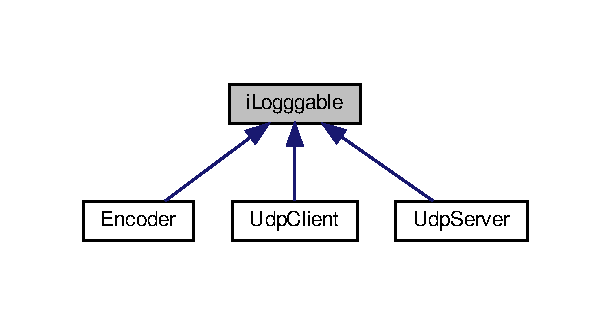
\includegraphics[width=293pt]{classi_logggable__inherit__graph}
\end{center}
\end{figure}
\subsection*{Public Member Functions}
\begin{DoxyCompactItemize}
\item 
void \textbf{ error} (const char $\ast$msg)
\begin{DoxyCompactList}\small\item\em Log an error message. \end{DoxyCompactList}\item 
void \textbf{ log} (const char $\ast$msg)
\begin{DoxyCompactList}\small\item\em Log an ordinary message. \end{DoxyCompactList}\end{DoxyCompactItemize}


\subsection{Member Function Documentation}
\mbox{\label{classi_logggable_ae7bda22bccfb292f6d9be01d3b5aaeaf}} 
\index{i\+Logggable@{i\+Logggable}!error@{error}}
\index{error@{error}!i\+Logggable@{i\+Logggable}}
\subsubsection{error()}
{\footnotesize\ttfamily void i\+Logggable\+::error (\begin{DoxyParamCaption}\item[{const char $\ast$}]{msg }\end{DoxyParamCaption})\hspace{0.3cm}{\ttfamily [inline]}}



Log an error message. 


\begin{DoxyParams}{Parameters}
{\em msg} & The error message to log \\
\hline
\end{DoxyParams}
\mbox{\label{classi_logggable_abd81f07c9bacd1d223f6bf8d50c02e64}} 
\index{i\+Logggable@{i\+Logggable}!log@{log}}
\index{log@{log}!i\+Logggable@{i\+Logggable}}
\subsubsection{log()}
{\footnotesize\ttfamily void i\+Logggable\+::log (\begin{DoxyParamCaption}\item[{const char $\ast$}]{msg }\end{DoxyParamCaption})\hspace{0.3cm}{\ttfamily [inline]}}



Log an ordinary message. 


\begin{DoxyParams}{Parameters}
{\em msg} & The message to log \\
\hline
\end{DoxyParams}


The documentation for this class was generated from the following file\+:\begin{DoxyCompactItemize}
\item 
headers/log.\+h\end{DoxyCompactItemize}

\section{Udp\+Client Class Reference}
\label{class_udp_client}\index{Udp\+Client@{Udp\+Client}}


Inheritance diagram for Udp\+Client\+:\nopagebreak
\begin{figure}[H]
\begin{center}
\leavevmode
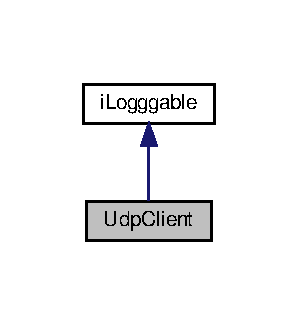
\includegraphics[width=143pt]{class_udp_client__inherit__graph}
\end{center}
\end{figure}


Collaboration diagram for Udp\+Client\+:\nopagebreak
\begin{figure}[H]
\begin{center}
\leavevmode
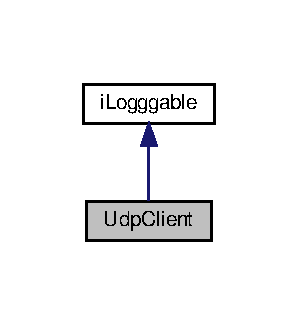
\includegraphics[width=143pt]{class_udp_client__coll__graph}
\end{center}
\end{figure}
\subsection*{Public Member Functions}
\begin{DoxyCompactItemize}
\item 
\textbf{ Udp\+Client} (const int \&P\+O\+RT)
\begin{DoxyCompactList}\small\item\em Construct a new Udp Client object. \end{DoxyCompactList}\item 
bool \textbf{ send} (const std\+::string \&input)
\begin{DoxyCompactList}\small\item\em Send a message over a U\+DP socket. \end{DoxyCompactList}\end{DoxyCompactItemize}


\subsection{Constructor \& Destructor Documentation}
\mbox{\label{class_udp_client_a36317032b2a10d0d3f9db6be7f8ef37c}} 
\index{Udp\+Client@{Udp\+Client}!Udp\+Client@{Udp\+Client}}
\index{Udp\+Client@{Udp\+Client}!Udp\+Client@{Udp\+Client}}
\subsubsection{Udp\+Client()}
{\footnotesize\ttfamily Udp\+Client\+::\+Udp\+Client (\begin{DoxyParamCaption}\item[{const int \&}]{P\+O\+RT }\end{DoxyParamCaption})\hspace{0.3cm}{\ttfamily [inline]}}



Construct a new Udp Client object. 


\begin{DoxyParams}{Parameters}
{\em P\+O\+RT} & The port to send the message to \\
\hline
\end{DoxyParams}


\subsection{Member Function Documentation}
\mbox{\label{class_udp_client_adff031651eb312a55b66bc4ac52627a0}} 
\index{Udp\+Client@{Udp\+Client}!send@{send}}
\index{send@{send}!Udp\+Client@{Udp\+Client}}
\subsubsection{send()}
{\footnotesize\ttfamily bool Udp\+Client\+::send (\begin{DoxyParamCaption}\item[{const std\+::string \&}]{input }\end{DoxyParamCaption})}



Send a message over a U\+DP socket. 


\begin{DoxyParams}{Parameters}
{\em input} & std\+::string \\
\hline
\end{DoxyParams}
\begin{DoxyReturn}{Returns}
true If the U\+DP transmission worked 

false If the U\+DP transmission failed 
\end{DoxyReturn}


The documentation for this class was generated from the following files\+:\begin{DoxyCompactItemize}
\item 
headers/udpclient.\+h\item 
udpclient.\+cpp\end{DoxyCompactItemize}

\section{Udp\+Server Class Reference}
\label{class_udp_server}\index{Udp\+Server@{Udp\+Server}}


Inheritance diagram for Udp\+Server\+:\nopagebreak
\begin{figure}[H]
\begin{center}
\leavevmode
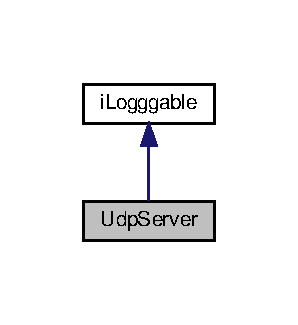
\includegraphics[width=143pt]{class_udp_server__inherit__graph}
\end{center}
\end{figure}


Collaboration diagram for Udp\+Server\+:\nopagebreak
\begin{figure}[H]
\begin{center}
\leavevmode
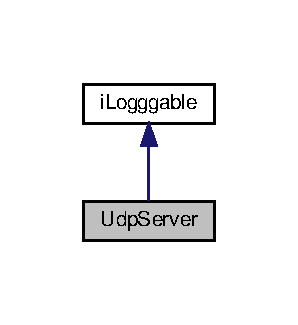
\includegraphics[width=143pt]{class_udp_server__coll__graph}
\end{center}
\end{figure}
\subsection*{Public Member Functions}
\begin{DoxyCompactItemize}
\item 
\textbf{ Udp\+Server} (const int port)
\begin{DoxyCompactList}\small\item\em Construct a new Udp Server object. \end{DoxyCompactList}\item 
bool \textbf{ serve} ()
\begin{DoxyCompactList}\small\item\em Start the U\+DP server. \end{DoxyCompactList}\item 
void \textbf{ on\+Message} (const std\+::string \&message)
\begin{DoxyCompactList}\small\item\em The message handler when a U\+DP message is recieved on the U\+DP server. \end{DoxyCompactList}\end{DoxyCompactItemize}


\subsection{Constructor \& Destructor Documentation}
\mbox{\label{class_udp_server_abb91737f6586814939681baabb0cf9c7}} 
\index{Udp\+Server@{Udp\+Server}!Udp\+Server@{Udp\+Server}}
\index{Udp\+Server@{Udp\+Server}!Udp\+Server@{Udp\+Server}}
\subsubsection{Udp\+Server()}
{\footnotesize\ttfamily Udp\+Server\+::\+Udp\+Server (\begin{DoxyParamCaption}\item[{const int}]{port }\end{DoxyParamCaption})}



Construct a new Udp Server object. 


\begin{DoxyParams}{Parameters}
{\em port} & The port to start the server on \\
\hline
\end{DoxyParams}


\subsection{Member Function Documentation}
\mbox{\label{class_udp_server_a71fcac42f7f8592434c6c1b580b1506c}} 
\index{Udp\+Server@{Udp\+Server}!on\+Message@{on\+Message}}
\index{on\+Message@{on\+Message}!Udp\+Server@{Udp\+Server}}
\subsubsection{on\+Message()}
{\footnotesize\ttfamily void Udp\+Server\+::on\+Message (\begin{DoxyParamCaption}\item[{const std\+::string \&}]{message }\end{DoxyParamCaption})}



The message handler when a U\+DP message is recieved on the U\+DP server. 


\begin{DoxyParams}{Parameters}
{\em message} & The Message recieved on the U\+DP socket \\
\hline
\end{DoxyParams}
\mbox{\label{class_udp_server_a44bb69c6b92e55c2a667514b33782aef}} 
\index{Udp\+Server@{Udp\+Server}!serve@{serve}}
\index{serve@{serve}!Udp\+Server@{Udp\+Server}}
\subsubsection{serve()}
{\footnotesize\ttfamily bool Udp\+Server\+::serve (\begin{DoxyParamCaption}{ }\end{DoxyParamCaption})}



Start the U\+DP server. 

\begin{DoxyReturn}{Returns}
true If the U\+DP is live and amd exited gracefully (somehow) 

false If the U\+DP server could not be started 
\end{DoxyReturn}


The documentation for this class was generated from the following files\+:\begin{DoxyCompactItemize}
\item 
headers/udpserver.\+h\item 
main.\+cpp\item 
udpserver.\+cpp\end{DoxyCompactItemize}

%--- End generated contents ---

% Index
\backmatter
\newpage
\phantomsection
\clearemptydoublepage
\addcontentsline{toc}{chapter}{Index}
\printindex

\end{document}
